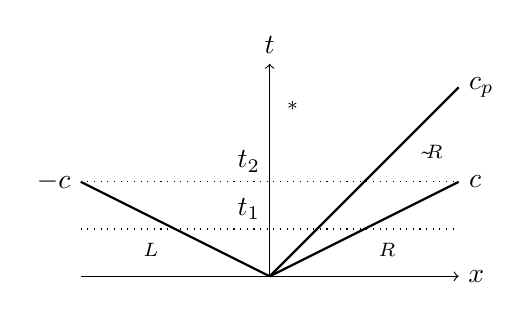
\begin{tikzpicture}[scale=0.6]
  \draw[->] (-4,0) -- (4.,0) node[right] {$x$};
  \draw[->] (0,0) -- (0,4.5) node[above] {$t$};
  \draw[thick] (0,0) -- (4.,2) node [right] {$c$};
  \draw[thick] (0,0) -- (4.,4) node [right] {$c_p$};
  \draw[thick] (0,0) -- (-4.,2) node [left] {$-c$};
  %\draw[thick] (0,0) -- (-4.,4) node [left] {$-c_p$};
  \draw[dotted] (-4,1.)-- (0,1) node [above left] {$t_1$} --(4.,1);
  \draw[dotted] (-4,2.)-- (0,2) node [above left] {$t_2$} --(4.,2);
  \node at (-2.5,0.) [above]{$\Qcb^L$};
  \node at (+2.5,0.) [above] {$\Qcb^R$};
  %\node at (-3.5,2.5) {$\tilde{\Qcb}^L$};
  \node at (+3.5,2.5) {$\tilde{\Qcb}^R$};
  \node at (0.5,3.5)  {$\Qcb^*$};
\end{tikzpicture}

%%% Local Variables:
%%% mode: latex
%%% TeX-master: "../../mainManuscript"
%%% End: